\section{Verification purpose}

\textbf{Case ID:} \CaseID

This case verifies statistical convergence of the stochastic smoldering-to-flaming (SFT) model and the resulting ignition-probability response. Pooled ignition-delay samples must converge to the configured SFT scale, while ensemble-mean firebrand-driven spread must respond consistently to ignition probability.

The test exposes biased sampling, insufficient ensemble size, incorrect delay extraction, and grid-dependent probability application. Success is determined from confidence-aware delay statistics and declared ensemble metrics, never from a single realization.

\section{Mathematical formulation and numerical implementation}
For accumulated firebrands in a cell, ELMFIRE's SIMPLE model uses
\begin{equation}
 F(t)=1-(1-P)^{t/\tau}, \qquad
 P_{\Delta t}=1-(1-P)^{\Delta t/\tau},
 \label{eq:cdf}
\end{equation}
where $P=P_{\mathrm{ign,small}}$, $\tau=\tau_{\mathrm{ign}}$, and
$P_{\Delta t}$ is the Bernoulli probability evaluated during one solver step.
Consequently $F(\tau)=P$: at $P=0.9$, the theoretical 90th percentile is
$q_{0.9}=\tau=10$~s. A successful local transition is followed by
\texttt{CELL\_IGNITION\_DELAY}=0, so the final TOA records the full ignition
time without an additional development lag.

For the dedicated delay members, transient ember-flux output is written every
wind-CFL step. If a cell's first nonzero transient flux occurs at dump $k$, its
first deposition lies in $(t_{k-1},t_k]$. Postprocessing uses the interval
midpoint $t_{d,i}=(t_{k-1}+t_k)/2$ and forms the actual-output sample
\begin{equation}
 d_i=t_{\mathrm{ign},i}-t_{d,i}.
 \label{eq:delay}
\end{equation}
Only centerline cells marked in the final ember-ignition raster, outside the
two-cell halo and in the 155--2800~m complete-support interval, are admitted.
The dump spacing $\Delta t$ is retained as the temporal-censoring resolution.

For the response sweep,
\begin{equation}
 CFL_w=\frac{u_w\Delta t}{\Delta x}=0.5,
 \qquad r_m=\frac{R_m}{u_w},
 \label{eq:ros}
\end{equation}
and each member ROS $R_m$ is the least-squares slope of centerline distance
against final TOA over 100--2800~m. Ten explicit seeds are paired across
$\Delta x=5,10,20,30$~m and $P=0,0.25,0.5,0.75,1$.

\section{Derivation of expected behavior}
Equation~\ref{eq:cdf} gives the exact event-level expectation
$q_{0.9}=10$~s. A finite sample quantile fluctuates, but its bootstrap confidence
interval should contract as independently seeded members add cell samples. The
final pooled estimate should therefore approach 10~s rather than an ROS-derived
surrogate. Timestep-resolved deposition limits the deterministic timing
uncertainty to the deposition interval.

At $P=0$, the ignition hazard is zero, and no spotting-driven front should
propagate. Increasing $P$ increases $F(t)$ for every $t>0$ and therefore cannot
reduce population-mean ROS. At $P=1$, ignition is immediate in the continuous
model and $\overline r$ should approach one. Because physical extent and
$CFL_w$ are fixed, the four resolution curves should nearly coincide.

\section{Verification metrics and acceptance criteria}
For every response group with $N=10$, the postprocessor calculates the mean,
sample standard deviation, standard error, and two-sided Student-$t$ 95\%
confidence interval. Adjacent probability means may decrease only within their
pooled confidence half-widths. At each $P$, the spread of the four resolution
means must not exceed 0.10, and every $P=1$ mean must be at least 0.90.

For the delay ensemble, samples are pooled after each independent member. At the
final member, all ten members must be usable, at least 1000 delays must be
available, $|\widehat q_{0.9}-10~\mathrm{s}|\le1$~s, and the 2000-replicate
bootstrap 95\% interval half-width must not exceed 1~s. A missing final TOA,
ignition map, dump-time table, transient sequence, stale raster shape, or empty
sample set makes that member incomplete. Overall PASS is the conjunction of all
response and delay components; missing required output yields
\texttt{insufficient\_output}, never a pass.

\subsection{Justification of metric quantification}

A two-sided 95\% Student-\(t\) interval is used because each response mean has
only ten independent ensemble members and its variance is estimated from those
members.  Allowing an adjacent decrease only within the pooled confidence
half-width distinguishes sampling noise from evidence against monotonicity
without assuming equal variances.  The 0.10 cross-resolution range and the
0.90 unit-probability floor each represent ten percentage points on the
naturally normalized \([0,1]\) response scale: they admit finite-ensemble and
grid-crossing variability but reject a practically material resolution effect
or failure to approach immediate ignition.

The target \(q_{0.9}=\SI{10}{s}\) follows directly from the prescribed SFT
distribution~\cite{Qin2025}.  Requiring 1000 pooled delays gives substantial
support in the upper decile rather than allowing a few extreme samples to set
the quantile.  The \SI{1}{s} accuracy and bootstrap-half-width limits are each
10\% of the model timescale, so both bias and uncertainty must be small on the
scale being verified.  Two thousand bootstrap replicates provide stable
percentile endpoints for this engineering decision without treating the
bootstrap interval as an exact physical confidence bound.  Full member
completeness is required because silently dropping failed stochastic runs can
bias both response means and delay quantiles.

\subsection{Predeclared acceptance contract}

Table~\ref{tab:acceptance-contract} summarizes the metrics fixed before
inspection of the calculated results. Numerical values and component statuses
are reported separately in Section~7.

\begin{table}[H]
\centering
\footnotesize
\caption{Predeclared verification metrics and acceptance criteria.}
\label{tab:acceptance-contract}
\begin{tabular}{@{}p{0.23\linewidth}p{0.47\linewidth}p{0.21\linewidth}@{}}
\toprule
Metric & Output, region, and aggregation & Acceptance criterion\\
\midrule
Response-ensemble completeness & Ten usable members for every resolution--probability group. & 200 of 200 members \\
Probability monotonicity & Adjacent ensemble-mean normalized ROS differences, allowing decrease only within pooled 95\% confidence half-widths. & Every adjacent check passes \\
Resolution spread & Range of the four resolution means at each ignition probability. & \(\le0.10\) \\
Unit-probability response & Minimum ensemble-mean normalized ROS at \(P_{ign}=1\). & \(\ge0.90\) \\
SFT sample completeness & Ten usable delay members and pooled interval-censored ignition-delay samples. & 10 members and at least 1000 samples \\
SFT 90th percentile & Absolute difference between pooled \(\widehat q_{0.9}\) and the configured \SI{10}{s} scale. & \(\le\SI{1}{s}\) \\
SFT uncertainty & Half-width of the 2000-replicate bootstrap 95\% interval for \(\widehat q_{0.9}\). & \(\le\SI{1}{s}\) \\
Overall decision & Conjunction of every response and SFT component; incomplete output is not evaluable. & PASS only if all pass \\
\bottomrule
\end{tabular}
\end{table}

\section{Simulation configuration and predicted outcome}

Figure~\ref{fig:input-configuration} records the prepared spatial inputs for \texttt{dx10\_pign0p5\_r01}.
The postprocessor reads these panels from the variant-local GeoTIFF files, removes the
two-cell numerical buffer, and retains map coordinates in metres.  The left panel shows
the most informative fuel or structure layout available for the case; the right panel
shows the cells selected by the non-positive initial level-set field, making a localized
ignition or firebrand-emission source explicit.

\begin{figure}[H]
\centering

\includegraphics[width=0.98\textwidth,height=0.42\textheight,keepaspectratio]{../figures/input_configuration.pdf}
\caption{Whole-domain prepared input configuration for the representative variant.  The
physical domain is shown without the numerical halo; coordinates, configured wind values,
fuel or structure layout, and initial ignition/source geometry are identified in the panels.}
\label{fig:input-configuration}
\end{figure}

\begin{table}[htbp]
\centering\small
\begin{tabular}{p{0.22\textwidth}p{0.23\textwidth}p{0.13\textwidth}p{0.30\textwidth}}
\toprule
Parameter & Configured value & Unit & Verification role \\
\midrule
Physical domain & $3600\times300$ & m & Fixed physical extent \\
Buffer & 2 cells per side & cells & Excluded numerical halo \\
Response grids & 5, 10, 20, 30 & m & Resolution comparison \\
Delay grid & 10 & m & delay-ensemble spatial baseline \\
Wind & 15 (6.7056) & mph (m/s) & Uniform transport \\
Wind CFL & 0.5 & -- & Fixed $\Delta t/\Delta x$ \\
Stop time & 240 & s & Common observation window \\
Response probabilities & 0, 0.25, 0.50, 0.75, 1 & -- & probability-response design \\
Delay model & $P=0.9$, $\tau=10$ & --, s & delay-distribution design \\
Ensembles & $20\times10$ response; 10 delay & runs & Sampling statistics \\
Generation & PER-AREA, 10 & pcs m$^{-2}$ s$^{-1}$ & No-surface source \\
Accumulation/ignition & EULERIAN/SIMPLE & -- & Implementation under test \\
Surface/development delay & disabled/0 & --, s & Isolate SFT waiting time \\
Delay output cadence & one wind-CFL step & s & Bracket first deposition \\
\bottomrule
\end{tabular}
\caption{Configuration of the merged ensemble-convergence case verification.}
\end{table}

The predicted response plot contains four nondecreasing curves beginning at zero
and approaching one. The delay plot should approach the horizontal 10~s line,
with its sampling interval narrowing as ensemble members are pooled.

\section{Actual simulation results}

Figure~\ref{fig:domain-result} shows the representative ember-ignition field from \texttt{dx10\_pign0p5\_r01}.
It is read from the actual ELMFIRE output named in the panel, masks nodata, and excludes
the two-cell numerical buffer.  This representative ensemble member supplies spatial evidence alongside the ensemble probability and delay statistics; it is not used as a replacement for those statistical metrics.

\begin{figure}[H]
\centering

\includegraphics[width=0.96\textwidth,height=0.50\textheight,keepaspectratio]{../figures/domain_result.pdf}
\caption{Whole-domain ember-ignition field from the representative completed ELMFIRE run.  This
domain-scale result supplements, rather than replaces, the higher-level verification
profiles, convergence plots, ensemble statistics, and calculated acceptance metrics below.}
\label{fig:domain-result}
\end{figure}


The distribution-level ignition-delay check is presented first because it
compares the sampled stochastic variable directly with its prescribed model
quantile. Figure~\ref{fig:delay-distribution} uses only delays reconstructed
from actual arrival-time, ember-ignition, dump-time, and transient-flux outputs.

\begin{figure}[H]
\centering
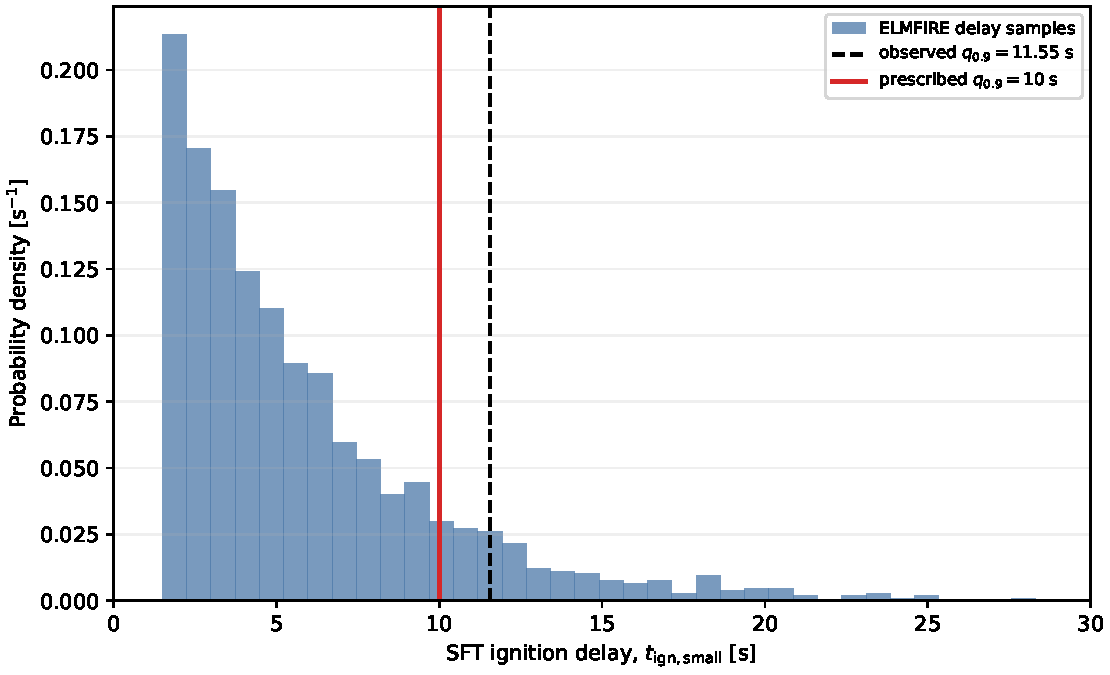
\includegraphics[width=0.82\textwidth,height=0.46\textheight,keepaspectratio]{../figures/sft_delay_distribution.pdf}
\caption{Probability density of sampled SFT ignition delays. The solid red line
is the prescribed 90th percentile and the dashed black line is the observed
pooled 90th percentile.}
\label{fig:delay-distribution}
\end{figure}

Figure~\ref{fig:response} presents the second reference observable: the
ensemble-mean normalized leading-edge ROS response to ignition probability and
spatial resolution.

\begin{figure}[H]
\centering
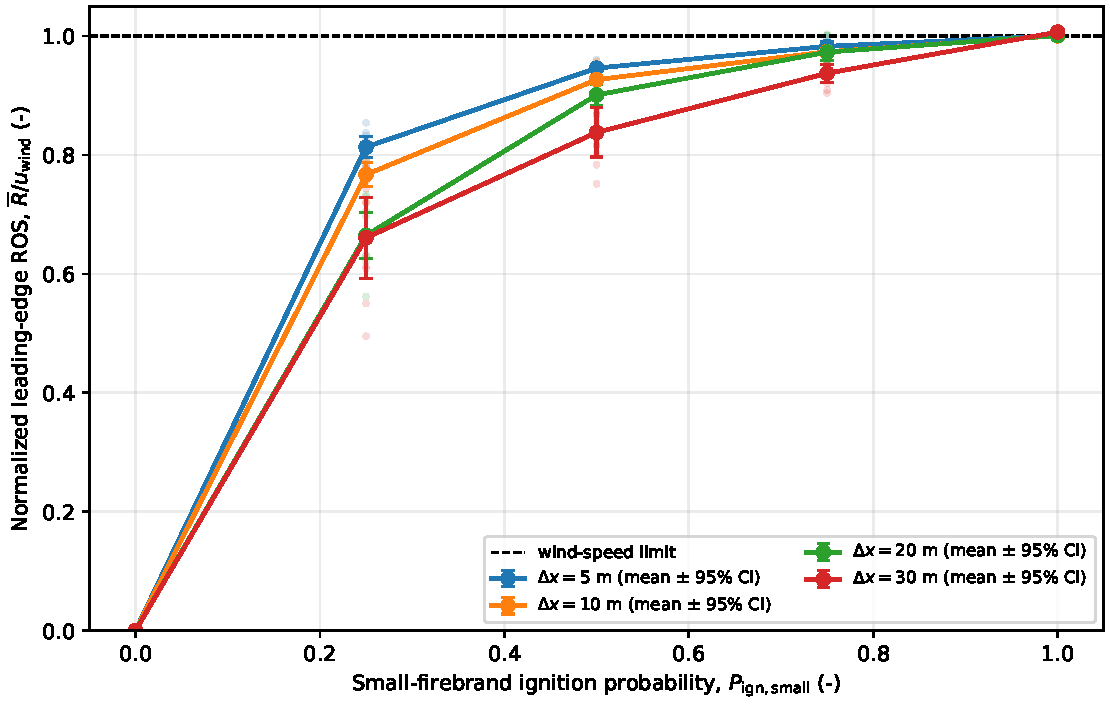
\includegraphics[width=0.94\textwidth,height=0.55\textheight,keepaspectratio]{../figures/ignition_probability_convergence.pdf}
\caption{Ensemble-mean normalized leading-edge ROS versus
$P_{\mathrm{ign,small}}$. Error bars are 95\% confidence intervals and faint
points are independently seeded ELMFIRE members.}
\label{fig:response}
\end{figure}

Figure~\ref{fig:delay} is an additional sample-size diagnostic. It shows how
the pooled delay quantile and its bootstrap uncertainty change as independent
members are added.

\begin{figure}[H]
\centering
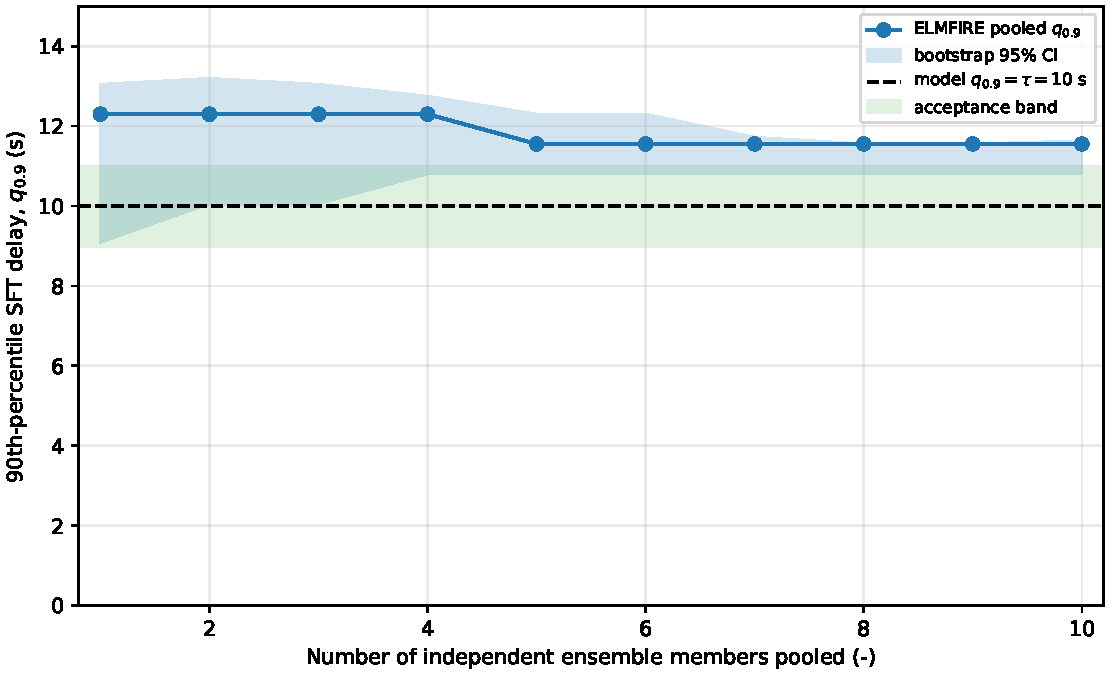
\includegraphics[width=0.82\textwidth,height=0.46\textheight,keepaspectratio]{../figures/sft_delay_ensemble_convergence.pdf}
\caption{Cumulative convergence of the pooled ELMFIRE 90th-percentile SFT
delay. The dashed line is the model expectation, blue shading is the bootstrap
95\% interval, and the green band is the $\pm1$~s acceptance interval.}
\label{fig:delay}
\end{figure}

\section{Calculated metrics and verification decision}
\begin{table}[htbp]
\centering\small
\begin{tabular}{p{0.42\textwidth}p{0.25\textwidth}p{0.22\textwidth}}
\toprule
Metric & Requirement & Calculated \\
\midrule
Response members & 200 usable & \Metric{evaluatedmembers}/\Metric{requiredmembers} \\
Probability response & monotone within 95\% uncertainty & \Metric{monotonewithuncertainty} \\
Maximum resolution-mean spread & $\le0.10$ & \Metric{maxcrossresolutionmeanspread} \\
Minimum $P=1$ mean & $\ge0.90$ & \Metric{minimump1mean} \\
SFT members & 10 usable & \Metric{evaluatedsftmembers}/\Metric{requiredsftmembers} \\
SFT delay samples & $\ge1000$ & \Metric{sftdelaysamples} \\
SFT 90th percentile & $10\pm1$ s & \Metric{sftobservedquantiles} s \\
SFT quantile absolute error & $\le1$ s & \Metric{sftquantileabsoluteerrors} s \\
SFT bootstrap half-width & $\le1$ s & \Metric{sftbootstrapci95halfwidths} s \\
SFT component & all delay checks pass & \Metric{sftdelaypassed} \\
Overall status & all components pass & \textbf{\Metric{status}} \\
\bottomrule
\end{tabular}
\caption{Metrics read directly from \texttt{outputs/metrics.json}.}
\end{table}
The machine-readable overall decision is \textbf{\Metric{verificationpassed}}.

\section{Technical interpretation}
The response ensemble currently has \Metric{evaluatedmembers}/\Metric{requiredmembers}
usable members. Its maximum cross-resolution spread is
\Metric{maxcrossresolutionmeanspread}, so that component can be distinguished
from the stochastic-delay check. The dedicated delay ensemble currently has
\Metric{evaluatedsftmembers}/\Metric{requiredsftmembers} usable members and
\Metric{sftdelaysamples} admitted delays. Therefore the merged case status is
\textbf{\Metric{status}} until every required component is evaluable and passes.
This separation prevents a plausible ROS curve from masking an incorrect SFT
waiting-time distribution, and prevents a correct quantile from masking
grid-sensitive propagation.

\section{Scope and limitations}
The case verifies one SIMPLE SFT time scale, one delay probability, one uniform
wind and fuel, Eulerian accumulation, zero full-development delay, and the
specified grid/probability sweep. Midpoint reconstruction of first deposition is
interval-censored at one wind-CFL step; that resolution is recorded but is not
sampling uncertainty. Cell samples within a run share a propagating fire history,
so independent run count and pooled cell count are both reported. The test does
not validate the empirical choice of $P$ or $\tau$, physical ignition thresholds,
surface-fire competition, PHYSICAL ignition, Lagrangian transport, or firebrand
consumption.

\begin{thebibliography}{9}
\bibitem{Qin2025}
Y. Qin, \emph{A Physics-Based Eulerian Framework for Modeling Firebrand
Showering in Regional-Scale Wildland and Wildland--Urban Interface Fire
Simulations}, Ph.D. dissertation, University of Maryland, College Park, 2025.
\end{thebibliography}
